\documentclass[11pt,a4paper]{article}
\usepackage[a4paper,top=2.35cm,bottom=2.35cm,left=2.35cm,right=2.35cm]{geometry}
\usepackage[T1]{fontenc}
\usepackage[utf8]{inputenc}
\usepackage[english]{babel}
\usepackage{lmodern}
\usepackage{microtype}
\usepackage{graphicx}
\usepackage{xcolor}
\usepackage{booktabs}
\usepackage{tabularx}
\usepackage{array}
\usepackage{float}
\usepackage{fvextra}
\usepackage[colorlinks=true,allcolors=black]{hyperref}

\graphicspath{{outputs/figures/}}

\newcommand{\mavg}{\textit{m.avg}}
\newcommand{\Mavg}{\textit{M.avg}}
\newcommand{\code}[1]{\texttt{#1}}

\begin{document}

\pagenumbering{gobble}
\begin{titlepage}
    \centering
    \vspace*{3cm}
    {\huge Aspect Based Sentiment Analysis \par}
    \vspace{2.3cm}
    {\Large \itshape Roger Baiges Trilla \par}
    \vspace{0.2cm}
    {\Large \itshape Guillem Olivart Garrofé \par}
    \vspace{2.3cm}
    {\Large Universitat Politècnica de Catalunya \par}
    \vspace{0.2cm}
    {\Large School of Informatics of Barcelona \par}
    \vspace{0.5cm}
    {\large Large Language Models \par}
    \vfill
    {\large Lluís Màrquez Villodre \par}
    \vspace{1.3cm}
    {\large May 2026 \par}
\end{titlepage}
\clearpage
\pagenumbering{arabic}

\section{Experimental Setup and Data Diagnostics}

The project consists of four required stages: zero-shot prompting, few-shot prompting, synthetic data augmentation, and fine-tuning. We treated all of them as the same constrained generation task: for each bilingual restaurant review, the model must emit a JSON object whose keys belong to the 11 valid aspect categories and whose values belong to the four valid polarities. A prediction is useful only if both the aspect and the polarity are correct, so the task is not just sentiment classification; it is structured extraction with a closed schema.

Our main generator was \textit{Qwen3.5-2B}. We selected it instead of the older model suggested in the starter code because it is a newer small open model, it is multilingual, it has a chat template suitable for instruction following, and it can be run repeatedly on a single 3090-class GPU. This mattered because the project required many full devel-set experiments, not just a single final run. For retrieval-based few-shot prompting we used \textit{Qwen3-Embedding-0.6B}, keeping the generator and retriever in the same model family while using a much smaller model for dense retrieval.

All model selection was performed on \code{devel.json}, exactly as the assignment defines this split: it is the validation set used to make prompt, decoding, retrieval, and checkpoint decisions. The held-out test set was not used during development. We therefore report all numbers on devel and keep the final conclusions explicitly validation-based.

The official scoring script treats each predicted aspect--polarity pair as one item. We report \mavg{} F1, the global micro-F1 over all predicted and gold pairs, and \Mavg{} F1, the average of per-review F1 scores. This distinction matters: \mavg{} rewards recovering frequent labels, while \Mavg{} is more sensitive to reviews with few or rare labels. We also track exact match accuracy, because the final output is a complete structured object and one extra or missing label makes the whole review different from the gold JSON. Precision and recall are interpreted at pair level: over-generating plausible aspects hurts precision, while omitting rare aspects hurts recall.

\begin{table}[H]
    \centering
    \small
    \setlength{\tabcolsep}{5pt}
    \caption{Dataset shape. English reviews contain more labels per review, while Spanish dominates the number of examples.}
    \label{tab:dataset_shape}
    \begin{tabular}{@{}llrrrr@{}}
        \toprule
        Split & Language & Reviews & Labels & Labels/review & Empty reviews \\
        \midrule
        Train & all & 1056 & 3748 & 3.55 & 29 \\
        Train & Spanish & 713 & 2360 & 3.31 & 29 \\
        Train & English & 343 & 1388 & 4.05 & 0 \\
        Devel & all & 132 & 454 & 3.44 & 3 \\
        Devel & Spanish & 91 & 285 & 3.13 & 3 \\
        Devel & English & 41 & 169 & 4.12 & 0 \\
        \bottomrule
    \end{tabular}
\end{table}

\begin{figure}[H]
    \centering
    \begin{minipage}{0.49\textwidth}
        \centering
        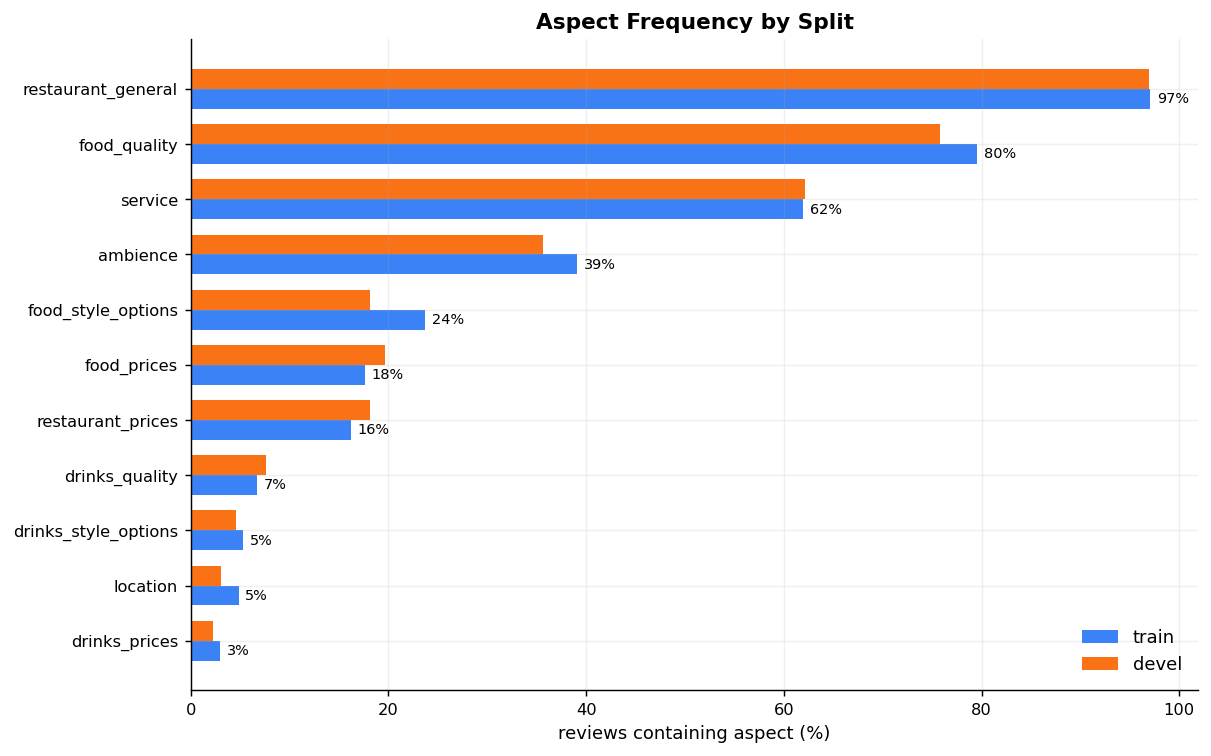
\includegraphics[width=\linewidth]{aspect_frequency.png}
    \end{minipage}
    \hfill
    \begin{minipage}{0.49\textwidth}
        \centering
        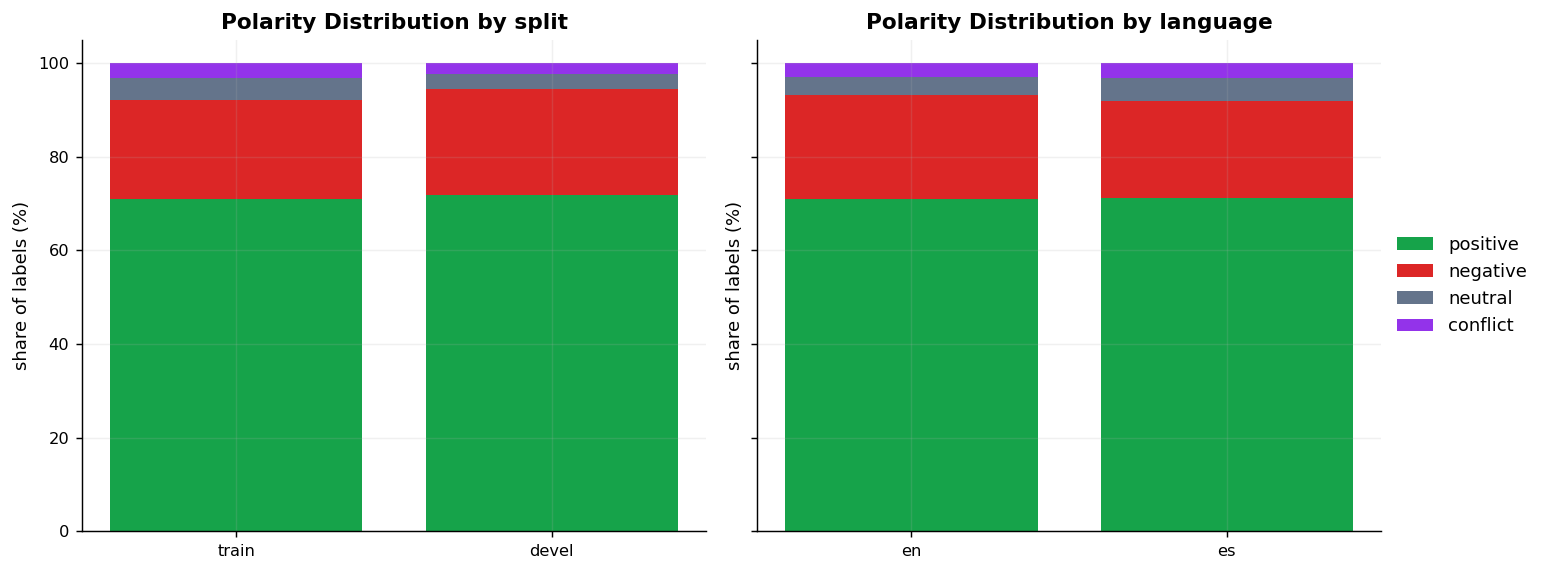
\includegraphics[width=\linewidth]{polartiy_distribution.png}
    \end{minipage}
    \caption{The corpus is dominated by frequent positive labels for \code{restaurant\_general}, \code{food\_quality}, and \code{service}. Price, drinks, style/options, neutral, and conflict labels form the long tail.}
    \label{fig:data_distribution}
\end{figure}

The distribution in Figure~\ref{fig:data_distribution} drove most design decisions. A model can obtain a non-trivial score by predicting common positive aspects, but the useful part of the task lies in controlling over-prediction and recovering rare boundaries such as restaurant-level prices versus food prices, food quality versus food style/options, and neutral/conflict polarity. This is why we did not optimize only for the highest number of predicted labels: the best system must decide when an aspect is genuinely mentioned, not merely probable in a restaurant review.

The imbalance is not only global but also multilingual. In devel, Spanish contains no \code{drinks\_style\_options} gold label, while English contains all six of them. Conversely, most neutral/conflict cases are Spanish. This made language-aware retrieval and language-balanced synthetic generation important: optimizing only the global score can hide failures in the smaller English split or in the Spanish rare-polarity cases.

The number of labels per review also shaped the generation limits. Empty reviews exist, but most examples contain several labels. Therefore, a valid prompt cannot ask for exactly one sentiment, and a valid decoding configuration cannot simply stop after the first pair. At the same time, the gold JSON is short compared with the instruction prompt, which later becomes important for loss masking during fine-tuning. The correct target distribution is compact multi-label JSON, not long natural-language explanations.

Before running LLM experiments we used these observations to define three diagnostic checks for every output file. First, we counted predicted labels against gold labels to detect over-generation or under-generation. Second, we kept raw generations separately from parsed predictions so malformed JSON could be inspected rather than silently discarded. Third, we broke down errors by aspect and language, because a small increase in global F1 can hide large regressions in long-tail labels.

\section{Baselines, Zero-Shot Prompting, and Decoding}

We first implemented frequency baselines to quantify how much the training distribution alone explains. These baselines do not read the review; they only exploit the marginal label distribution in \code{train.json}. This is a useful sanity check because the corpus is skewed enough that a naive majority predictor can appear moderately strong.

The strongest legal frequency baseline, \code{top3\_majority}, always predicts the three most frequent aspect--polarity pairs from the training set and reaches 56.24 \mavg{} F1. Predicting more labels increases recall but quickly destroys precision: \code{top8\_majority} sees more gold labels, but its micro-F1 falls to 41.7. The oracle baseline, which uses the gold devel aspects and only guesses polarity by majority class, reaches 71.80 \mavg{} F1. This isolates aspect detection as the harder part: if aspects were known, polarity would be much easier.

\begin{table}[H]
    \centering
    \small
    \setlength{\tabcolsep}{5pt}
    \caption{Frequency baselines. The gap between \code{top3\_majority} and the oracle shows that detecting mentioned aspects is harder than assigning their majority polarity.}
    \label{tab:baseline_family}
    \begin{tabular}{@{}lrrrr@{}}
        \toprule
        Baseline & P & R & \Mavg{} F1 & \mavg{} F1 \\
        \midrule
        Empty & 0.0 & 0.0 & 0.0 & 0.0 \\
        \code{top1\_positive} & 72.0 & 27.2 & 36.9 & 32.4 \\
        \code{top3\_majority} & 60.4 & 56.8 & 55.6 & 56.2 \\
        \code{top4\_majority} & 51.9 & 63.4 & 54.5 & 55.8 \\
        \code{top8\_majority} & 29.8 & 70.7 & 40.5 & 41.7 \\
        Oracle aspects + majority polarity & 72.6 & 72.6 & 72.6 & 71.8 \\
        \bottomrule
    \end{tabular}
\end{table}

\begin{table}[H]
    \centering
    \small
    \setlength{\tabcolsep}{4pt}
    \caption{Main zero-shot progression on the development set.}
    \label{tab:zeroshot}
    \begin{tabular}{@{}lrrrrrr@{}}
        \toprule
        System & Pred. & Gold & P$_\mu$ & R$_\mu$ & \Mavg{} F1 & \mavg{} F1 \\
        \midrule
        Empty baseline & 0 & 454 & 0.00 & 0.00 & 0.00 & 0.00 \\
        \code{top3\_majority} & 396 & 454 & 60.35 & 52.64 & 55.64 & 56.24 \\
        Zero-shot prompt v1 & 646 & 454 & 39.78 & 56.61 & 46.90 & 46.73 \\
        Zero-shot prompt v2 & 355 & 454 & 63.10 & 49.34 & 53.86 & 55.38 \\
        Best zero-shot sweep & 383 & 454 & 74.67 & 63.00 & 67.93 & 68.34 \\
        Oracle aspects + majority polarity & 454 & 454 & 71.81 & 71.81 & 72.60 & 71.81 \\
        \bottomrule
    \end{tabular}
\end{table}

The first prompt failed mostly by over-generation: it produced 646 labels for 454 gold labels and treated implicit or absent aspects as if they should still be emitted. The second prompt explicitly forbade using \code{neutral} for ``not mentioned'', clarified when \code{restaurant\_general} should appear, and required strict quoted JSON values. This fixed the worst hallucination pattern, but made the model too conservative. We therefore separated prompt design from decoding search and tuned generation parameters after stabilizing the prompt.

The final zero-shot prompt family followed four principles. First, it describes the closed schema in operational terms, especially the difference between absent aspects and neutral polarity. Second, it tells the model to output only JSON, without explanations, markdown, or confidence scores. Third, it treats \code{restaurant\_general} as a real expressed opinion, not as a default label that should always be present. Fourth, it makes empty JSON valid when no aspect is evaluated. These details matter more than wording style: most early failures came from ambiguous task boundaries, not from lack of sentiment knowledge.

The prompt finally used for the rest of the project was \code{absa\_v6}, shown in Appendix~\ref{appendix:prompt_v6}. It was intentionally dataset-aware but not example-biased. Instead of inserting a hand-picked review, it uses aggregate priors from the training split as search hints: \code{restaurant\_general}, \code{food\_quality}, \code{service}, and \code{ambience} are named as common categories, while drinks, prices, style/options, and location are described as valid but evidence-dependent categories. This was the key compromise between v1 and v2. The model is encouraged to recover the common labels that devel reviews often contain, but every label still needs textual support.

\begin{table}[H]
    \centering
    \small
    \setlength{\tabcolsep}{4pt}
    \caption{Main design elements of \code{absa\_v6}. The prompt is shown in full in Appendix~\ref{appendix:prompt_v6}.}
    \label{tab:prompt_v6_design}
    \begin{tabularx}{\textwidth}{@{}lX@{}}
        \toprule
        Prompt block & Purpose \\
        \midrule
        Strict output contract & Forces exactly one JSON object with quoted valid aspect and polarity strings. \\
        Dataset-aware priors & Raises recall for frequent aspects without adding demonstrations or leaking devel examples. \\
        Recall rule & Prevents the overly conservative v2 behavior by reminding the model that long reviews often contain several labels. \\
        Neutral/conflict rules & Separates explicit neutral sentiment from absent aspects, and reserves conflict for mixed sentiment on the same aspect. \\
        Aspect mapping hints & Turns ambiguous wording such as value, portions, waiting, decor, wine list, or parking into the correct closed aspect. \\
        Completeness checklist & Makes the model do one final pass over food, service, ambience, prices, drinks, location, and unsupported labels. \\
        \bottomrule
    \end{tabularx}
\end{table}

Later prompt variants, especially \code{absa\_v8}, tried to make the wording more balanced, but they did not replace \code{absa\_v6} as the project anchor. The reason is practical: \code{absa\_v6} was the prompt used for the strongest hyperparameter search, the few-shot experiments, and the fine-tuning format. Keeping the same prompt across stages made comparisons meaningful. Otherwise an apparent improvement from few-shot or fine-tuning could partly be a prompt-format change rather than a true method improvement.

The best zero-shot region was not the official Qwen sampling recipe. For this extraction task, the best setting was more conservative: temperature 0.65, top-p 0.75, top-k 20, presence penalty 2.0, repetition penalty 1.0, and max-new-tokens 512. This improved the official-like setup from 55.87 to 68.34 \mavg{} F1.

\begin{table}[H]
    \centering
    \small
    \setlength{\tabcolsep}{4pt}
    \caption{Representative decoding sweep after the prompt was fixed to \code{absa\_v6}.}
    \label{tab:decoding}
    \begin{tabular}{@{}lrrrrrr@{}}
        \toprule
        Config & Temp. & Top-p & Top-k & PP & \Mavg{} F1 & \mavg{} F1 \\
        \midrule
        Official-like & 1.00 & 1.00 & 20 & 2.0 & 55.53 & 55.87 \\
        No presence penalty & 1.00 & 1.00 & 20 & 0.0 & 56.74 & 59.47 \\
        Conservative & 0.70 & 0.80 & 20 & 1.5 & 65.20 & 66.12 \\
        Refined & 0.70 & 0.80 & 20 & 1.8 & 66.64 & 68.18 \\
        Best single run & 0.65 & 0.75 & 20 & 2.0 & 67.93 & 68.34 \\
        \bottomrule
    \end{tabular}
\end{table}

The sweep shows that the model needs restraint, not open-ended diversity. Presence penalty is useful before fine-tuning because it discourages repetitive lists and helps the model stop adding the same common labels, but too much sampling makes the model enumerate plausible restaurant aspects instead of extracting only the expressed ones. We also checked narrower configurations close to greedy decoding, but before fine-tuning they tended to lose recall: the base model had not yet internalized the extraction format, so a small amount of stochasticity helped recover labels that greedy decoding missed.

Optuna was useful mostly as an organized local search rather than as a fully automated optimizer. Because each devel run was expensive, we did not run a huge combinatorial grid over prompts, $K$, temperature, top-p, and top-k. Instead, we fixed a good prompt, tested coherent decoding regions, inspected their errors, and then refined around the best region. This kept the number of experiments linear and interpretable: every new run answered a specific question about precision, recall, or stability.

We also tested Qwen thinking mode, but it was unusable for the main pipeline: in an 8-example pilot with a 4096-token budget, only 2 generations closed \code{<think>}, 6 hit the limit, and the run produced only 2 predicted labels over 22 gold labels. The model was not mainly looping; it was spending the whole budget deliberating about definitions and never emitting the final JSON.

Malformed JSON was not the dominant zero-shot failure after prompt v2, but we kept a conservative parser repair step for common JSON-like outputs such as unquoted polarity values. The raw string is stored, then the evaluator parses a normalized prediction. The repair only accepts valid aspect names and valid polarity values; it does not invent labels and it does not map arbitrary free text to the closest aspect. This improved robustness without changing the semantic task. After this point, the dominant errors were semantic: missing rare aspects, confusing price scopes, and collapsing neutral/conflict into positive or negative.

\section{Few-Shot Prompting}

The few-shot stage used \code{train.json} demonstrations only; no devel examples were ever used as prompt examples. We compared random fixed examples, pure dense retrieval, a manually curated hard bank, a hard/retrieved mix, and an ABSA-aware MMR reranker. The final strategy, \code{absa\_mmr}, retrieves dense candidates with Qwen3-Embedding-0.6B and reranks them using semantic similarity, same-language preference, aspect-cue coverage, rare-label usefulness, length/label-count fit, and a diversity term. This was designed to avoid the common failure of semantic retrieval: selecting several near-duplicate positive restaurant reviews that do not teach rare aspects.

The selection problem is more important than it may look. A random few-shot prompt often teaches the model the majority distribution again, while a purely manual bank cannot adapt to the query. Dense retrieval is much better, but nearest neighbors can be too similar to each other: for example, a query about a positive dinner can retrieve several examples about positive food and service while missing the price or style boundary that actually matters. Our reranker therefore scores a candidate not only by similarity to the current review, but also by how much new ABSA information it adds relative to the examples already selected.

\begin{table}[H]
    \centering
    \small
    \setlength{\tabcolsep}{4pt}
    \caption{Exploration-stage few-shot comparison for $K=5$, seed 42. Retrieval quality matters more than simply adding examples.}
    \label{tab:fewshot_exploration}
    \begin{tabular}{@{}lrrrrr@{}}
        \toprule
        Method & Pred. & P$_\mu$ & R$_\mu$ & \Mavg{} F1 & \mavg{} F1 \\
        \midrule
        \code{dense\_topk} & 381 & 80.4 & 68.4 & 72.4 & 72.3 \\
        \code{absa\_mmr} & 388 & 79.1 & 68.5 & 72.0 & 71.7 \\
        \code{hard\_mix} & 392 & 74.7 & 65.7 & 68.4 & 68.3 \\
        \code{random\_fixed} & 412 & 74.7 & 65.8 & 67.5 & 67.4 \\
        \code{manual\_fixed\_hard} & 412 & 73.2 & 65.8 & 67.5 & 67.4 \\
        \bottomrule
    \end{tabular}
\end{table}

The $K=5$ exploration suggested that dense retrieval is already strong, but the final choice should not be based on one seed and one $K$. We therefore ran a confirmation stage over stronger $K$ values and multiple seeds. This is why the final few-shot result is not simply the best single exploration run: it is the setting that remained strong and stable when randomness changed.

\begin{table}[H]
    \centering
    \small
    \setlength{\tabcolsep}{4pt}
    \caption{Few-shot confirmation stage. Values are means over seeds 101, 202, and 303.}
    \label{tab:fewshot}
    \begin{tabular}{@{}lrrrrrr@{}}
        \toprule
        Method & K & P$_\mu$ & R$_\mu$ & \Mavg{} F1 & \mavg{} F1 & Std$_{\mavg}$ \\
        \midrule
        \code{absa\_mmr} & 8 & 79.60 & 69.02 & 73.85 & 73.93 & 0.50 \\
        \code{absa\_mmr} & 12 & 78.00 & 70.04 & 73.92 & 73.81 & 0.79 \\
        \code{dense\_topk} & 12 & 77.98 & 69.68 & 74.19 & 73.59 & 0.98 \\
        \code{dense\_topk} & 10 & 78.29 & 68.58 & 73.31 & 73.11 & 0.51 \\
        \bottomrule
    \end{tabular}
\end{table}

\code{absa\_mmr} with $K=8$ was selected as the best few-shot system because it had the best mean \mavg{} F1 and the lowest variance among the top configurations. Increasing to $K=12$ slightly improved recall but made the prompt less stable. The confirmed few-shot runs were mechanically clean: 100\% JSON parse success, no token-limit failures, and about 20 output tokens on average. The remaining errors were therefore semantic rather than formatting issues, mostly concentrated in \code{restaurant\_prices}, \code{food\_prices}, \code{food\_style\_options}, drinks aspects, and neutral/conflict polarity.

The language split exposed an additional retrieval effect. The selected $K=8$ ABSA-MMR configuration averaged 73.77 \mavg{} F1 in Spanish and 74.22 in English across the three seeds. English precision was higher, about 85.0 micro precision, but recall was lower because English reviews contain more labels per review. This justified keeping same-language matching as a soft score rather than a hard filter: cross-language examples can still be useful, but the default demonstrations should match the review language when possible.

The manual hard bank was still valuable as an analysis tool. It contained examples for empty reviews, mixed polarity, explicit neutral opinions, price/value complaints, style/options cues such as portions and variety, and cases where a review praises the restaurant globally but criticizes one concrete aspect. However, using only these fixed examples made the prompt less query-specific. The best compromise was to let retrieval choose the final demonstrations and encode the manual insights as reranking preferences rather than as a static prompt.

This stage also established an important ceiling for inference-only methods. Few-shot prompting moved from 68.34 to 73.93 \mavg{} F1, a clear gain, but the model still missed many long-tail labels. The remaining gap was no longer a formatting or demonstration-selection problem. It required changing the model weights so that the ABSA boundaries became part of the model's own decision function.

\section{Fine-Tuning Design}

Prompting and retrieval improved the model, but still left a large gap to the oracle baseline. We therefore fine-tuned Qwen3.5-2B with parameter-efficient adapters. The most important training detail was loss masking: the system prompt, user prompt, and any instruction text are masked with label value $-100$, so the loss is computed only on the assistant JSON answer. Without this, the prompt is much longer than the gold JSON and the model would spend most of its capacity learning to reproduce instructions instead of learning ABSA decisions.

We trained without few-shot examples in the SFT prompt. Few-shot prompting is an inference-time retrieval strategy; including demonstrations during training would change the input distribution and make the final model depend on long prompts. The final SFT format therefore matches the desired zero-shot inference format: instruction plus review text in, compact JSON out.

Both LoRA and QLoRA used rank 16, alpha 32, dropout 0.05, all linear Qwen projection modules, learning rate $10^{-4}$, cosine schedule, 5\% warmup, weight decay 0.01, max length 3072, and generative validation every 50 optimizer steps. The micro-batch was limited by GPU memory to 2 examples per device, so the effective batch size was controlled with gradient accumulation. QLoRA loads the base model in 4-bit and was the best training variant, reaching 87.35 \mavg{} F1. The max length was chosen from a token-budget notebook: \code{absa\_v6} plus compact gold JSON fits all train/devel examples below 3072 tokens, while dynamic padding avoids paying this length for every batch.

We did not create an additional validation split from \code{train.json}. The assignment explicitly defines \code{devel.json} as the split for development decisions, and the training set is already small. Holding out more train examples would reduce the supervision available for rare labels. Instead, the code trains on all of \code{train.json}, evaluates on devel every 50 optimizer steps, and keeps the checkpoint with the best generated ABSA F1. The final test set, once released, should be used only once with the selected checkpoint.

\begin{table}[H]
    \centering
    \small
    \setlength{\tabcolsep}{4pt}
    \caption{Training choices that differ from a minimal fine-tuning script.}
    \label{tab:training_design}
    \begin{tabularx}{\textwidth}{@{}lX@{}}
        \toprule
        Design choice & Reason \\
        \midrule
        Prompt loss masking & Prevents the long instruction prompt from dominating the short JSON target loss. \\
        No few-shot examples in SFT & Keeps training aligned with zero-shot fine-tuned inference and avoids dependence on retrieved demonstrations. \\
        Generative validation & Selects checkpoints by actual JSON extraction quality instead of teacher-forced token loss. \\
        Greedy fine-tuned inference & Removes sampling variance after the model has learned the structured output distribution. \\
        All-linear LoRA targets & Adapts attention and MLP projections without full-model training cost. \\
        \bottomrule
    \end{tabularx}
\end{table}

Loss masking is the main difference between a task-specific SFT setup and a naive chat fine-tuning setup. The prompt contains the complete aspect definitions, output constraints, and the review text; the target completion is usually a short JSON object. If the full sequence were supervised, most tokens in the loss would belong to the repeated prompt template. The model could obtain a low loss by learning to continue or copy instructions while paying relatively little attention to the scarce answer tokens. Masking the prompt makes every gradient update focus on the actual extraction decision: which aspect keys to include and which polarity value to assign.

This also explains why evaluation loss is not enough for model selection. A checkpoint can have slightly lower teacher-forced token loss because it assigns high probability to common JSON syntax, yet still produce worse generated outputs after decoding. ABSA is evaluated after parsing the generated object, so a single extra key, missing key, or wrong polarity has a discrete effect that token loss does not fully capture.

\begin{table}[H]
    \centering
    \small
    \setlength{\tabcolsep}{4pt}
    \caption{Best fine-tuned checkpoints on \code{devel.json}.}
    \label{tab:finetune}
    \begin{tabular}{@{}lrrrrrrr@{}}
        \toprule
        Run & Step & Pred. & OK & P$_\mu$ & R$_\mu$ & \Mavg{} F1 & \mavg{} F1 \\
        \midrule
        LoRA on train & 450 & 437 & 385 & 88.10 & 84.80 & 84.44 & 86.42 \\
        QLoRA on train & 400 & 439 & 390 & 88.84 & 85.90 & 85.29 & 87.35 \\
        Augmented PEFT on train+synthetic & 450 & 449 & 394 & 87.75 & 86.78 & 85.17 & 87.26 \\
        \bottomrule
    \end{tabular}
\end{table}

Checkpoint selection by validation loss would have chosen weaker models. For QLoRA, the minimum validation loss occurred at step 350 with 85.71 \mavg{} F1, while the best generative checkpoint was step 400 with 87.35. The difference is even clearer in the augmented run: the minimum loss was step 250 with 84.13 \mavg{} F1, but the best generated ABSA output was step 450 with 87.26. The loss values at steps 250 and 450 were almost identical, yet the task F1 differed by more than 3 points. We therefore selected checkpoints by full greedy generation on the development set, using \mavg{} F1 as the primary metric and \Mavg{} F1 as the tie-breaker.

\begin{table}[H]
    \centering
    \small
    \setlength{\tabcolsep}{4pt}
    \caption{Validation loss does not select the best ABSA checkpoint.}
    \label{tab:loss_vs_f1}
    \begin{tabular}{@{}lrrrr@{}}
        \toprule
        Run / checkpoint & Step & Eval loss & \Mavg{} F1 & \mavg{} F1 \\
        \midrule
        QLoRA, minimum loss & 350 & 0.1147 & 83.74 & 85.71 \\
        QLoRA, best generated F1 & 400 & 0.1204 & 85.29 & 87.35 \\
        Augmented, minimum loss & 250 & 0.1175 & 82.66 & 84.13 \\
        Augmented, best generated F1 & 450 & 0.1184 & 85.17 & 87.26 \\
        \bottomrule
    \end{tabular}
\end{table}

After fine-tuning, greedy decoding became the best inference policy. The sampling settings that helped zero-shot prompting were useful because the base model was under-calibrated for this extraction format and needed some exploration to recover missing labels. After SFT, the model has already learned the target JSON distribution; stochastic sampling mainly injects variance, extra labels, and polarity instability. Since ABSA extraction is a deterministic structured-output task, greedy decoding gives better reproducibility and preserves the decision boundary learned during fine-tuning.

For this reason, we did not reuse the zero-shot best decoding parameters for the final fine-tuned model. The zero-shot setting with temperature 0.65 and top-p 0.75 was a compensation mechanism for a base model that had not been trained on the ABSA schema. Once the model is supervised on gold JSON, the desired behavior is the most likely structured answer, not a sample from a distribution of plausible answers. Keeping sampling after SFT would make the same review produce slightly different label sets across runs, which is undesirable for a leaderboard-style extraction task.

\section{Targeted Synthetic Data Augmentation}

The assignment suggested generating many random synthetic reviews, but our best QLoRA checkpoint was already well calibrated: 439 predicted labels for 454 gold labels, no empty predictions on non-empty reviews, and no hallucinated predictions on empty-gold reviews. A large naive synthetic dataset risked damaging this calibration. We therefore generated a smaller targeted augmentation set of 220 examples.

The synthetic generation plan was driven by real QLoRA errors. We first ran the best QLoRA model on the training set and used its mistakes to identify hard regions: restaurant-level price judgments, food price versus restaurant price, food style/options, rare drinks aspects, ambience boundaries, and neutral/conflict polarity. Each train example received a difficulty score based on false negatives, false positives, polarity mistakes, rarity of the gold labels, and language. The development set was used only for aggregate diagnosis and final comparison; no devel review text was sent to the API or paraphrased.

Each synthetic example was generated by a strong API model from a controlled plan: target language, difficulty bucket, exact target gold dictionary, aspects to avoid, official aspect and polarity definitions, and three style examples selected from \code{train.json}. These style examples were not random; they were chosen to match language, share target aspects or aspect--polarity pairs, include cases difficult for the current model, and avoid excessive reuse. The API was not asked to label an arbitrary review; it was asked to write a natural review that realizes a specific gold JSON. This direction is important because it gives us direct control over the intended supervision signal.

The API response also had to include support spans, and a local validator required exact target-gold agreement, valid labels only, support-span presence, no annotation-like phrasing, and low n-gram similarity to train/devel examples. We accepted quality over quantity: rejected generations were not kept simply to reach a round number. This is why the final file contains 220 accepted examples rather than a large unfiltered synthetic corpus.

\begin{table}[H]
    \centering
    \small
    \setlength{\tabcolsep}{4pt}
    \caption{Final synthetic dataset composition.}
    \label{tab:synthetic}
    \begin{tabular}{@{}lrlr@{}}
        \toprule
        Bucket & Count & Language / shape & Count \\
        \midrule
        Price/value boundary & 56 & Spanish & 148 \\
        Food style/options boundary & 36 & English & 72 \\
        Ambience/location/service boundary & 30 & 0-label hard negatives & 11 \\
        Rare drinks aspects & 24 & 2-label examples & 36 \\
        Neutral/conflict polarity & 40 & 3-label examples & 143 \\
        Hard negatives / empty-gold & 14 & 4-label examples & 27 \\
        Natural regularizers & 20 & Total accepted & 220 \\
        \bottomrule
    \end{tabular}
\end{table}

The final training file was \code{train\_plus\_synthetic\_v1.shuffled.json}. Shuffling was intentional: the unshuffled file appended all 220 synthetic examples after the 1056 original examples, which could make late training steps disproportionately synthetic. The shuffled version preserves the exact same 1276-example multiset while distributing synthetic examples throughout the training order.

This design deliberately avoids using synthetic data as a replacement for the original corpus. The original train examples remain the majority and preserve the natural dataset distribution, while synthetic examples act as targeted local corrections. This is especially important for ABSA because nearby labels are easy to confuse: adding too many price examples can move the model from missing \code{restaurant\_prices} to overusing price labels in food-specific contexts.

\begin{figure}[H]
    \centering
    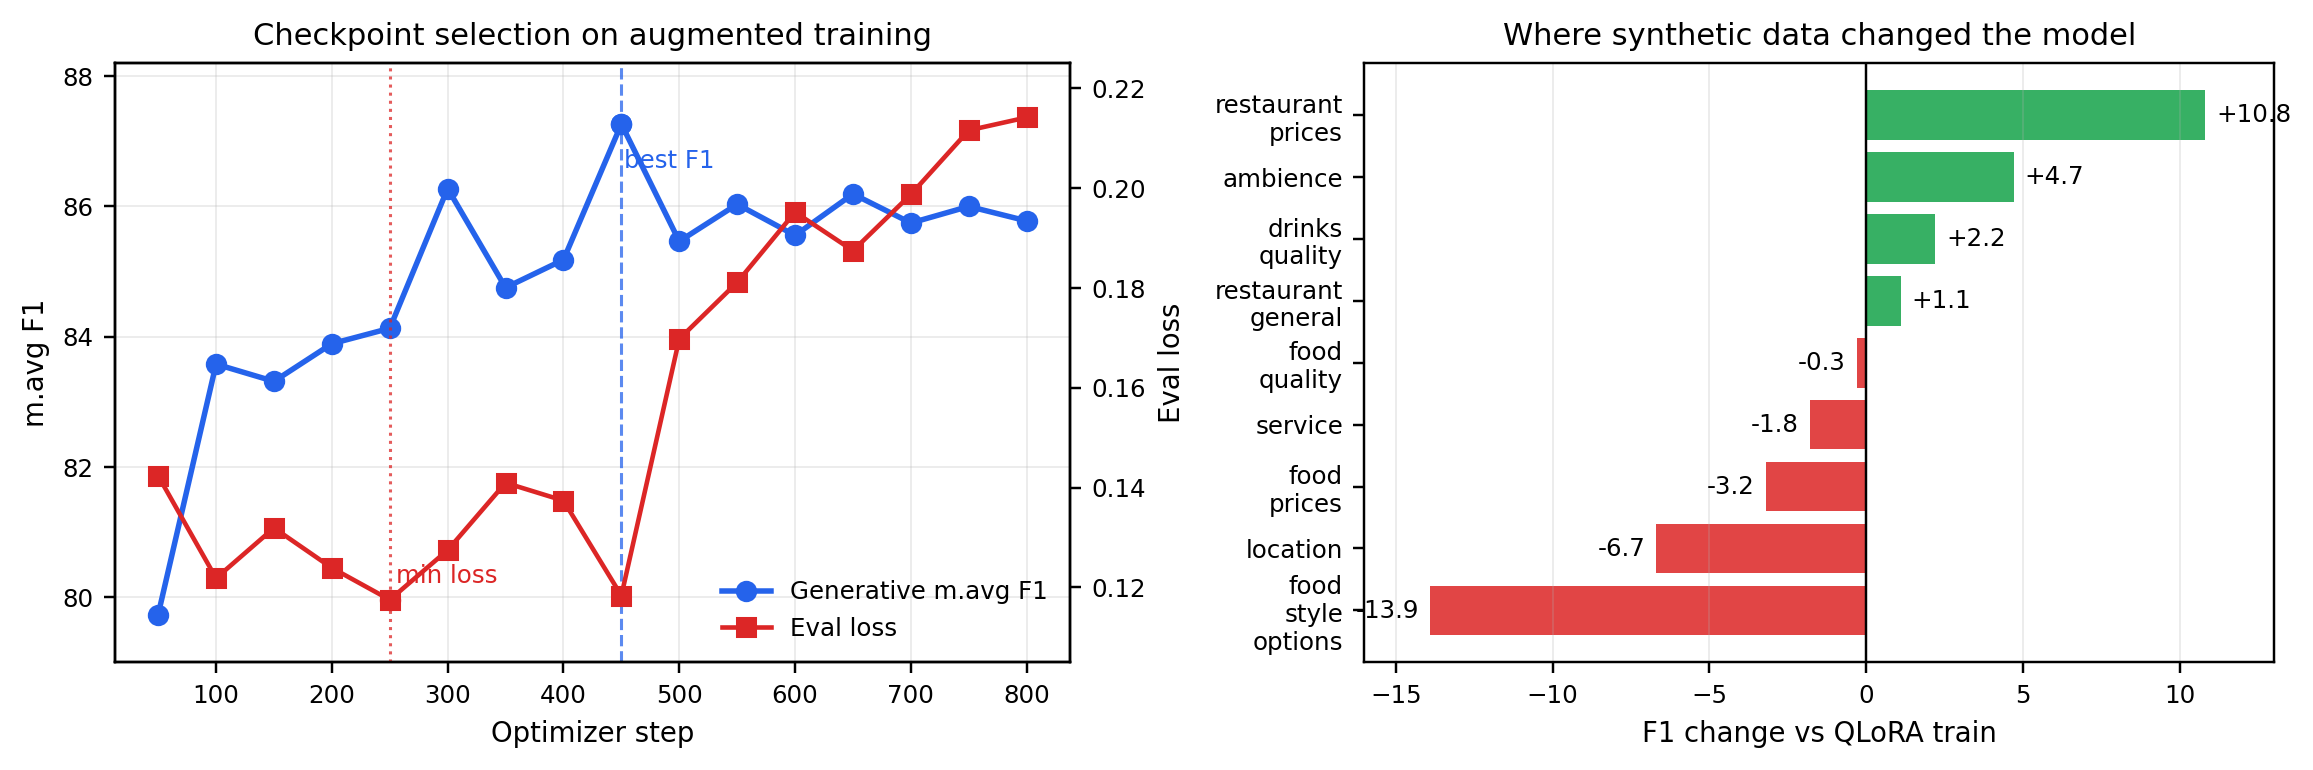
\includegraphics[width=0.96\textwidth]{final_ft_diagnostics.png}
    \caption{Synthetic augmentation did not improve the global best F1, but it changed useful boundaries. Left: validation loss would select a weaker checkpoint than generative F1. Right: the augmented model improves \code{restaurant\_prices} and \code{ambience}, but hurts nearby style/price boundaries.}
    \label{fig:ft_diagnostics}
\end{figure}

The augmented run is best interpreted as a controlled negative result. It did not beat the original QLoRA checkpoint globally: 87.26 versus 87.35 \mavg{} F1. However, it improved exact match accuracy from 73/132 to 76/132 and recovered more gold labels overall (394 versus 390 correct pairs). More importantly, the local effect matched part of the intended target: \code{restaurant\_prices} improved from 63.2 to 73.9 aspect-F1, \code{ambience} from 81.3 to 86.0, and \code{conflict} polarity from 28.6 to 42.1. These gains were offset by degradation in nearby categories, especially \code{food\_style\_options} (79.2 to 65.2), \code{food\_prices} (74.1 to 70.8), and \code{neutral} polarity (44.4 to 40.0). This shows that synthetic ABSA data can move decision boundaries, but controlling one boundary can destabilize another.

The most informative part is not the tiny global difference; it is the direction of the local changes. The augmentation succeeded where it was explicitly targeted, especially restaurant-level price/value and ambience cues. The cost appeared in adjacent labels that share vocabulary with the targets. For example, complaints about price can refer to the restaurant globally, to a specific dish, or to value-for-money in general. Similarly, food style/options overlaps with food quality when a review mentions portion size, variety, or presentation together with taste. The synthetic set therefore improved some intended boundaries but introduced pressure on related ones. This is exactly the type of trade-off that a final report should surface rather than hide.

\begin{table}[H]
    \centering
    \small
    \setlength{\tabcolsep}{5pt}
    \caption{Main local changes after synthetic augmentation, compared with the QLoRA train-only checkpoint.}
    \label{tab:synthetic_deltas}
    \begin{tabular}{@{}lrrrl@{}}
        \toprule
        Category & QLoRA F1 & Aug. F1 & Change & Interpretation \\
        \midrule
        \code{restaurant\_prices} & 63.2 & 73.9 & +10.8 & target boundary improved \\
        \code{ambience} & 81.3 & 86.0 & +4.7 & explicit atmosphere recovered \\
        \code{conflict} polarity & 28.6 & 42.1 & +13.5 & rare polarity improved \\
        \code{food\_prices} & 74.1 & 70.8 & -3.2 & price boundary shifted \\
        \code{neutral} polarity & 44.4 & 40.0 & -4.4 & still under-controlled \\
        \code{food\_style\_options} & 79.2 & 65.2 & -13.9 & style/quality boundary degraded \\
        \bottomrule
    \end{tabular}
\end{table}

\section{Language Robustness and Final Comparison}

The final models were balanced across languages despite the split imbalance. Spanish has more reviews, while English reviews contain more labels per example, making exact match harder. The best QLoRA checkpoint is slightly stronger in Spanish by \mavg{} F1, while the augmented model improves exact match in both languages.

\begin{table}[H]
    \centering
    \small
    \setlength{\tabcolsep}{4pt}
    \caption{Language-level results for the two strongest fine-tuned systems.}
    \label{tab:language}
    \begin{tabular}{@{}llrrrrr@{}}
        \toprule
        Model & Language & Gold & Pred. & \Mavg{} F1 & \mavg{} F1 & Exact \\
        \midrule
        QLoRA train & Spanish & 285 & 282 & 84.87 & 87.83 & 56/91 \\
        QLoRA train & English & 169 & 157 & 86.22 & 86.50 & 17/41 \\
        Augmented PEFT & Spanish & 285 & 286 & 84.42 & 87.92 & 58/91 \\
        Augmented PEFT & English & 169 & 163 & 86.85 & 86.14 & 18/41 \\
        \bottomrule
    \end{tabular}
\end{table}

The language-level numbers show that the final system is not simply overfitting to the majority Spanish split. The QLoRA model reaches 87.83 \mavg{} F1 in Spanish and 86.50 in English. The augmented run slightly improves Spanish \mavg{} and exact match, but slightly reduces English \mavg{} while still improving English exact match. This is consistent with the synthetic design: it was targeted at hard boundaries, not at a uniform language-level gain. Because English reviews contain more labels per review, one missing label has a stronger effect on exact match than on pair-level F1.

\begin{figure}[H]
    \centering
    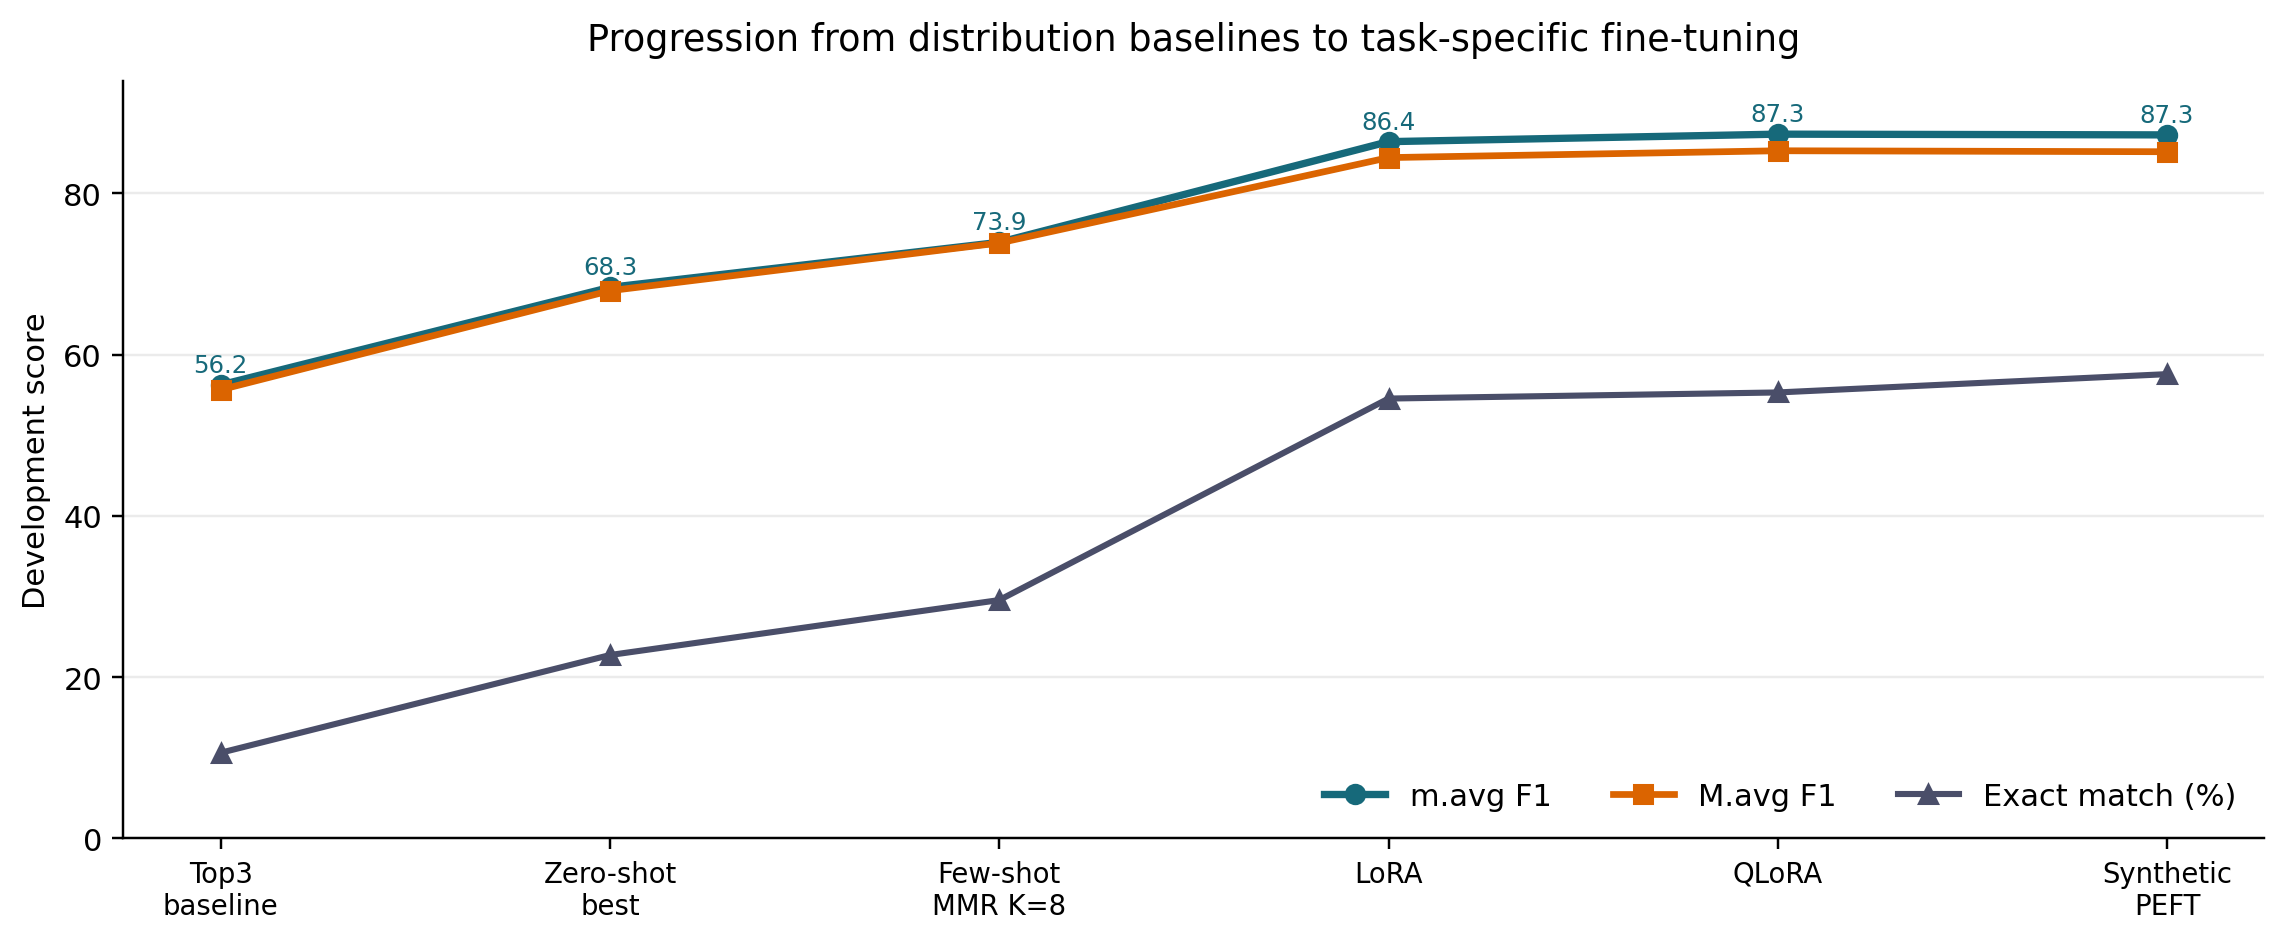
\includegraphics[width=0.96\textwidth]{final_stage_progression.png}
    \caption{Project-level progression. Prompting and decoding provide the first large gains, few-shot retrieval improves semantic coverage, and fine-tuning produces the decisive jump.}
    \label{fig:stage_progression}
\end{figure}

\begin{table}[H]
    \centering
    \small
    \setlength{\tabcolsep}{4pt}
    \caption{Main development-set results across the project.}
    \label{tab:final}
    \begin{tabular}{@{}lrrrrr@{}}
        \toprule
        System & P$_\mu$ & R$_\mu$ & \Mavg{} F1 & \mavg{} F1 & Exact \\
        \midrule
        \code{top3\_majority} baseline & 60.35 & 52.64 & 55.64 & 56.24 & 14/132 \\
        Best zero-shot sweep & 74.67 & 63.00 & 67.93 & 68.34 & 30/132 \\
        Best few-shot, \code{absa\_mmr}, $K=8$ & 79.60 & 69.02 & 73.85 & 73.93 & 39/132 \\
        LoRA on train & 88.10 & 84.80 & 84.44 & 86.42 & 72/132 \\
        QLoRA on train & \textbf{88.84} & 85.90 & \textbf{85.29} & \textbf{87.35} & 73/132 \\
        Augmented PEFT on train+synthetic & 87.75 & \textbf{86.78} & 85.17 & 87.26 & \textbf{76/132} \\
        \bottomrule
    \end{tabular}
\end{table}

The main lesson is that each stage solved a different bottleneck. Prompt engineering and decoding fixed formatting and over-generation; ABSA-aware few-shot retrieval improved coverage without fine-tuning; supervised adapters produced the large jump by internalizing the extraction format; generative-F1 checkpointing was necessary because token loss did not align with the evaluation metric; and synthetic data was useful diagnostically even though it did not improve the global score. The final system is therefore the QLoRA checkpoint selected by greedy generative validation, with the augmented run as evidence that targeted synthetic data can improve specific rare boundaries but must be controlled carefully to avoid shifting errors into related categories.

The remaining errors are no longer parser failures or broad hallucination. They are annotation-boundary errors: whether ``expensive for what it offers'' is a restaurant price or a food price, whether generous portions are food quality or style/options, whether a mixed review should be conflict or negative overall, and whether a short positive sentence implies \code{restaurant\_general} only or also a concrete aspect. These are exactly the decisions where a small local model benefits most from task-specific fine-tuning, but also where synthetic data must be generated with very precise controls.

If we had one more iteration, the most promising direction would not be a larger random synthetic set. The results suggest a narrower plan: generate fewer but more contrastive minimal pairs for the boundaries that moved in the wrong direction, especially \code{food\_prices} versus \code{restaurant\_prices}, \code{food\_quality} versus \code{food\_style\_options}, and neutral versus conflict. Each pair should keep the surface review similar while changing only the intended aspect or polarity. That would train the model on the exact distinctions that still fail, instead of increasing the amount of generic restaurant text.

\appendix
\section{Prompt \code{absa\_v6}}
\label{appendix:prompt_v6}

The following is the exact prompt file used as the project anchor for zero-shot tuning, few-shot prompting, and fine-tuning format. It is included here because small wording changes had measurable effects on recall and over-generation.

\VerbatimInput[
    fontsize=\scriptsize,
    breaklines=true,
    breakanywhere=true,
    frame=single
]{prompts/absa_v6_appendix.txt}

\end{document}
